\chapter{\large METHODOLOGY}
\thispagestyle{empty}
% -------- begin content from here--------

\section{System Specification} 

In this section, you are to document in details the characteristics of the input and output of the model of system you have developed. Provide the requirement for the input and the output by imposing restriction on the scopes of values or strings accepted and acceptable. Your will need to state assumptions that informs your requirements.

A specification should address the \textit{input} and \textit{output} of the problem-solving process, in the $Input \rightarrow$ \fbox{process()} $\rightarrow Output$ formulation. 

Example of circuit module digram for expressing hardware system specification is shown in Figure \ref{HarwareSpec}. Example of use case digram for expressing software system specification is shown in Figure \ref{usecase}. 

 
\begin{figure}[!h]
	\centering
	\fbox{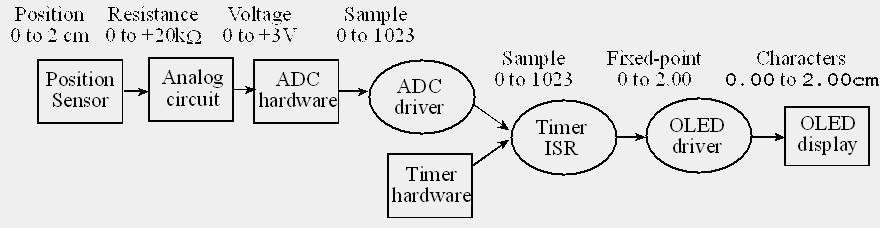
\includegraphics[scale=0.48]{HardWareSpec}}
	\caption{Hardware system specification}
	\label{HarwareSpec}
\end{figure}



\begin{figure}[!h]
	\centering
	\fbox{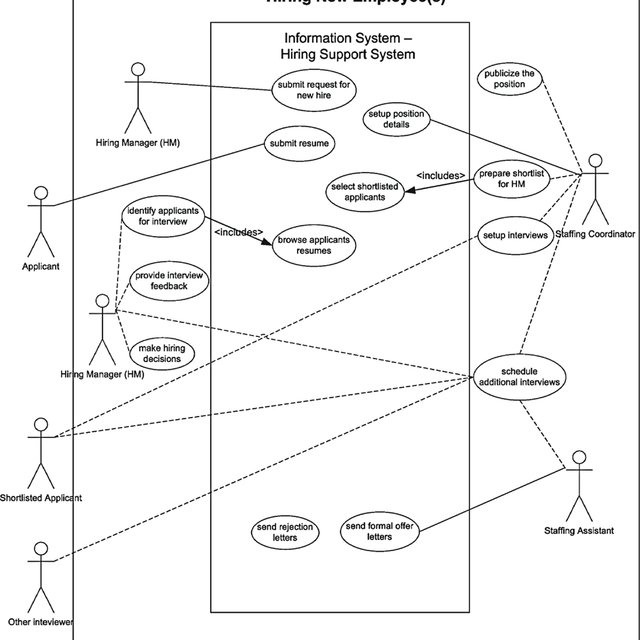
\includegraphics[scale=0.6]{Example-ofuse-case-diagram}}
	\caption{Use case diagram of system specification}
	\label{usecase}
\end{figure}





\section{Data Collection}
Data collected must be discussed in detail. An analysis of important data relevant for model formulation can be presented as depicted in Table \ref{tab-freq}. All table must be discussed in text. To do this, state what each column represents. Explain the first and the list items in the table as well as any other item that is interesting. For example, explain each item, or row, with largest or smallest values.

\begin{table}[!h]
	\caption{Special Characters in Research Data}
	\label{tab-freq}
	\centering
	\begin{tabular}{ccl}
		\hline \hline
		Symbols & Frequency & Comments\\
		\hline
		\d{O} & 1 in 1,000 & Found in \textit{Yor\`ub\'a}  names\\
		$\pi$ & 1 in 5 & Common in math\\
		\$ & 4 in 5 & Used in business\\
		$\Psi^2_1$ & 1 in 40,000 & Unexplained usage\\
		\hline\hline 
	\end{tabular}
\end{table}


\section{Model Formulation} 

In this section you are to document in details the symbolic representation and formulation of the inputs and the output as well as state the process by which the output is computed from the input using the process.
This is an example of in-text equation:
\begin{math}
\lim_{n\rightarrow \infty}x=0
\end{math}. In-text equations do not require reference numbering.

If the equation is in-line however, it must be placed on a line outside the text like Equation \ref{EquationInline} with unique reference number. The reference number must be used to discuss the equation in the text.


\begin{equation}
\lim_{n\rightarrow \infty}x=0
\label{EquationInline}
\end{equation}

Other examples of in-line equations are as presented in Equations \ref{Equationsam2}, \ref{Equationsam3} and \ref{Equationsam4}.

\begin{equation}
A_{m,n} = 
\begin{pmatrix}
a_{1,1} & a_{1,2} & \cdots & a_{1,n} \\
a_{2,1} & a_{2,2} & \cdots & a_{2,n} \\
\vdots  & \vdots  & \ddots & \vdots  \\
a_{m,1} & a_{m,2} & \cdots & a_{m,n} 
\end{pmatrix}
\label{Equationsam2}
\end{equation}



\begin{equation}
A = 
\begin{pmatrix}
1 & 2 & 3 \\
4 & 5 & 6 \\
7 & 8 & 9
\end{pmatrix}
\label{Equationsam3}
\end{equation}


\begin{equation}
|x| = \left\{
\begin{array}{rl}
-x & \text{if } x < 0,\\
0 & \text{if } x = 0,\\
x & \text{if } x > 0.
\end{array} \right.
\label{Equationsam4}
\end{equation}


\section{System Design} 

In this section, you are to document in details how you used design tools such as flowchart, UML diagrams, tree, entity relation diagram, sequence diagram, circuit diagram, timing diagram, etc. for the model or system. This include the design for data, user interface, program, hardware circuit, output, and so on.

The design of the structure of data using tree diagram should appear as depicted in Figure \ref{TreeTrans}. Every tree diagram must be discussed in the body of the text. For example in the case of Figure \ref{TreeTrans} you should state what the root, branches and leaves of the tree stands for and how you system will process a typical  input.

\begin{figure}[!h]
	\centering
\fbox{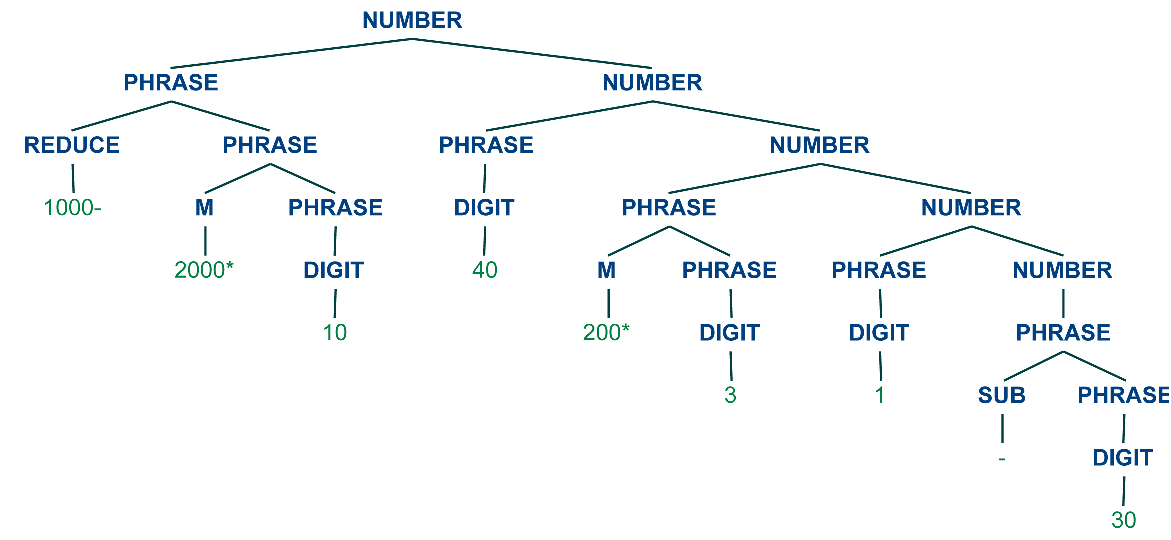
\includegraphics[scale=0.7]{tree3}}
	\caption{System Design Tree}
	\label{TreeTrans}
\end{figure}


Each algorithm can be represented in pseudocode as depicted in Algorithm 	\ref{alg:one}. For clarity, you may also set lines to identify the structure in your algorithm as shown in Algorithm 	\ref{alg:two}.

\begin{algorithm}[t]
\SetAlgoNoLine
	\KwIn{Node $\alpha$'s ID ($ID_{\alpha}$), and node $\alpha$'s
		neighbors' IDs within two communication hops.}
	\KwOut{The frequency number ($FreNum_{\alpha}$) node $\alpha$ gets assigned.}
	$index$ = 0; $FreNum_{\alpha}$ = -1\;
	\Repeat{$FreNum_{\alpha} > -1$}{
		$Rnd_{\alpha}$ = Random($ID_{\alpha}$, $index$)\;
		$Found$ = $TRUE$\;
		\For{each node $\beta$ in $\alpha$'s two communication hops
		}{
			$Rnd_{\beta}$ = Random($ID_{\beta}$, $index$)\;
			\If{($Rnd_{\alpha} < Rnd_{\beta}$) \text{or} ($Rnd_{\alpha}$ ==
				$Rnd_{\beta}$ \text{and} $ID_{\alpha} < ID_{\beta}$)\;
			}{
				$Found$ = $FALSE$; break\;
			}
		}
		\eIf{$Found$}{
			$FreNum_{\alpha}$ = $index$\;
		}{
			$index$ ++\;
		}
	}
	\caption{Frequency Number Computation}
	\label{alg:one}
\end{algorithm}




\begin{algorithm}[t]
	%	\SetAlgoNoLine
	\KwIn{Node $\alpha$'s ID ($ID_{\alpha}$), and node $\alpha$'s
		neighbors' IDs within two communication hops.}
	\KwOut{The frequency number ($FreNum_{\alpha}$) node $\alpha$ gets assigned.}
	$index$ = 0; $FreNum_{\alpha}$ = -1\;
	\Repeat{$FreNum_{\alpha} > -1$}{
		$Rnd_{\alpha}$ = Random($ID_{\alpha}$, $index$)\;
		$Found$ = $TRUE$\;
		\For{each node $\beta$ in $\alpha$'s two communication hops
		}{
			$Rnd_{\beta}$ = Random($ID_{\beta}$, $index$)\;
			\If{($Rnd_{\alpha} < Rnd_{\beta}$) \text{or} ($Rnd_{\alpha}$ ==
				$Rnd_{\beta}$ \text{and} $ID_{\alpha} < ID_{\beta}$)\;
			}{
				$Found$ = $FALSE$; break\;
			}
		}
		\eIf{$Found$}{
			$FreNum_{\alpha}$ = $index$\;
		}{
			$index$ ++\;
		}
	}
	\caption{Frequency Number Computation}
	\label{alg:two}
\end{algorithm}

Class digram for Object Oriented program design can be included as shown in Figure \ref{ClassDiag}.



\begin{figure}[!h]
	\centering
	\fbox{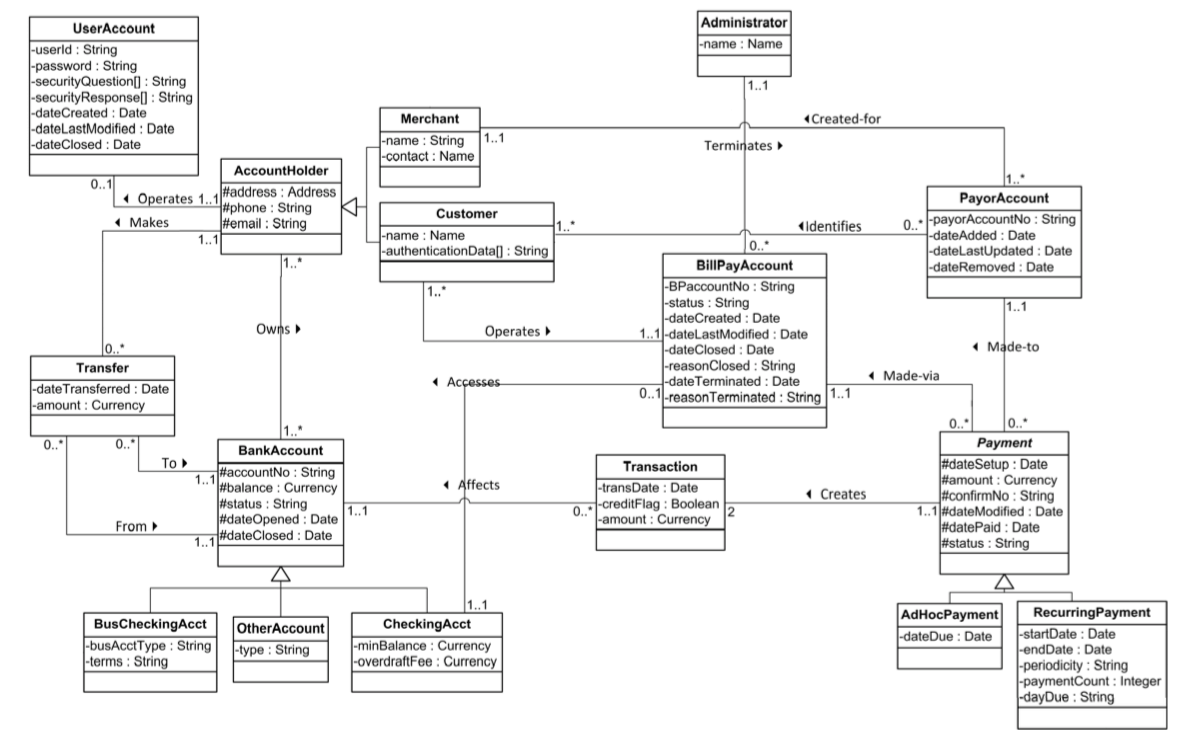
\includegraphics[angle=90, scale=0.5]{class-diagram}}
	\caption{Class diagram for OOP Program}
	\label{ClassDiag}
\end{figure}



A transition diagram should appear as depicted in Figure \ref{PdaTrans}. Every diagram must be discussed in the body of the text. For example in the case of Figure \ref{PdaTrans} you should state what each of the yellow circle stands for and how the machine will transit between states for a given input.

\begin{figure}[!h]
\centering
\fbox{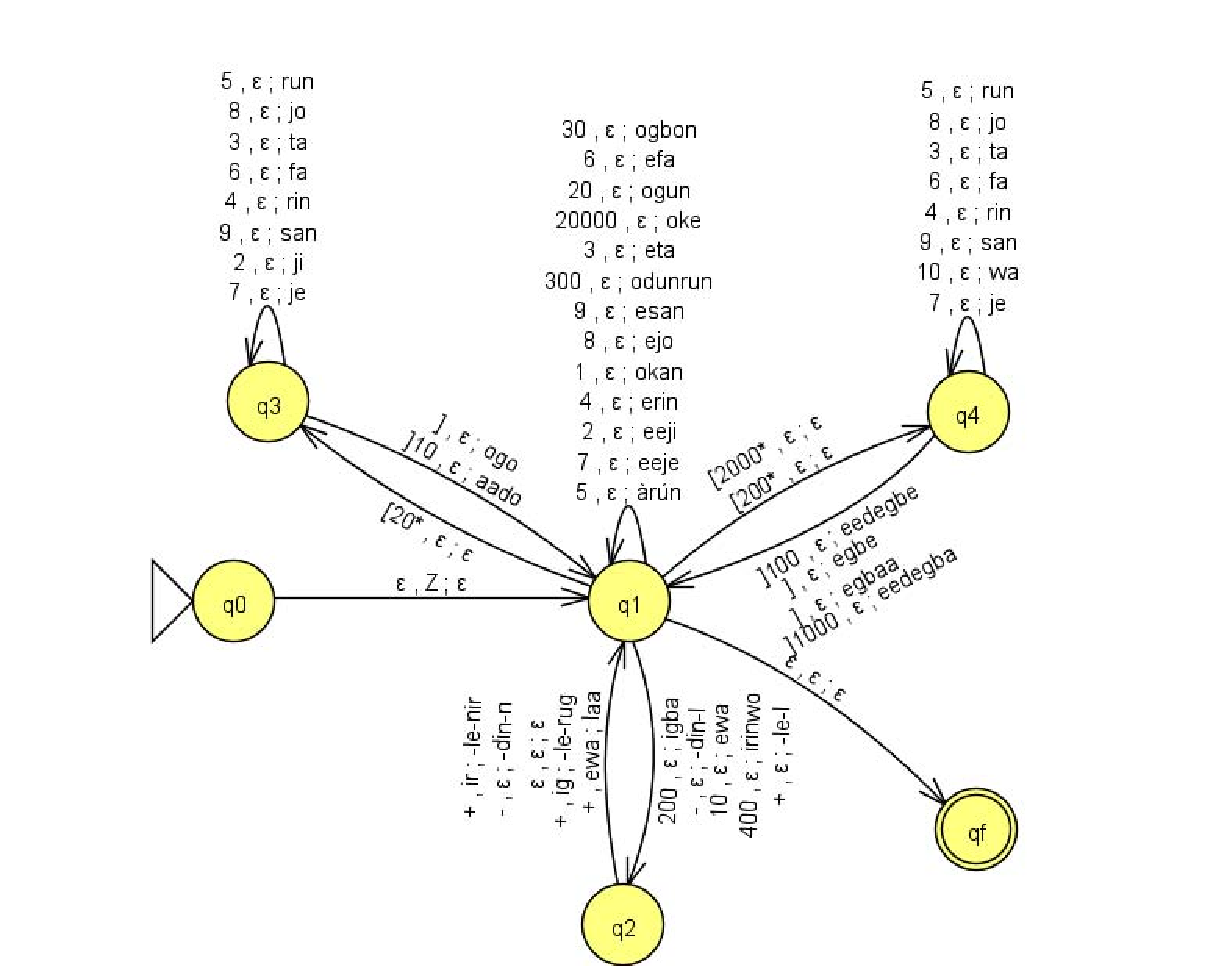
\includegraphics[scale=0.7]{pda}}
\caption{Transition Diagram for PDA}
\label{PdaTrans}
\end{figure}



A design algorithm represented using flowchart should be depicted as shown in Figure \ref{flochartExample}.

\begin{figure}
\centering
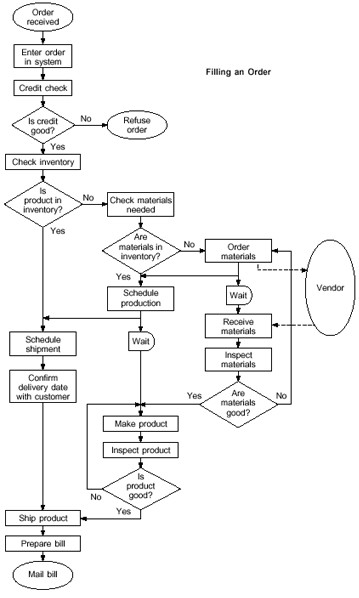
\includegraphics[scale=0.8]{flowchart-fig2}
\caption{Flowchart of Program Design}
\label{flochartExample}
\end{figure}


Hardware design can be presented as block digram in Figure \ref{BlokDiag}. 

\begin{figure}[!h]
	\centering
	\fbox{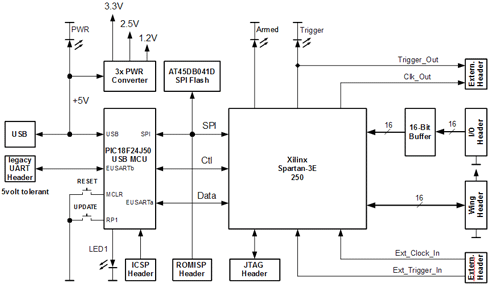
\includegraphics[scale=0.6]{blockDiagram}}
	\caption{Block diagram of hardware system}
	\label{BlokDiag}
\end{figure}

\section{System Implementation} You are now to document in details how you coded your program, did your simulation and/or hardware construction. The codes for the program modules that realise important aspects of your solution should be discussed here.

A user interface for the implemented program should appear as depicted in Figure \ref{dict2l}. Every such diagram must be discussed in the body of the text. For example in the case of Figure \ref{dict2l} you should discuss each section of the interface and state how the program will respond for a given input.

\begin{figure}[!h]
\centering
	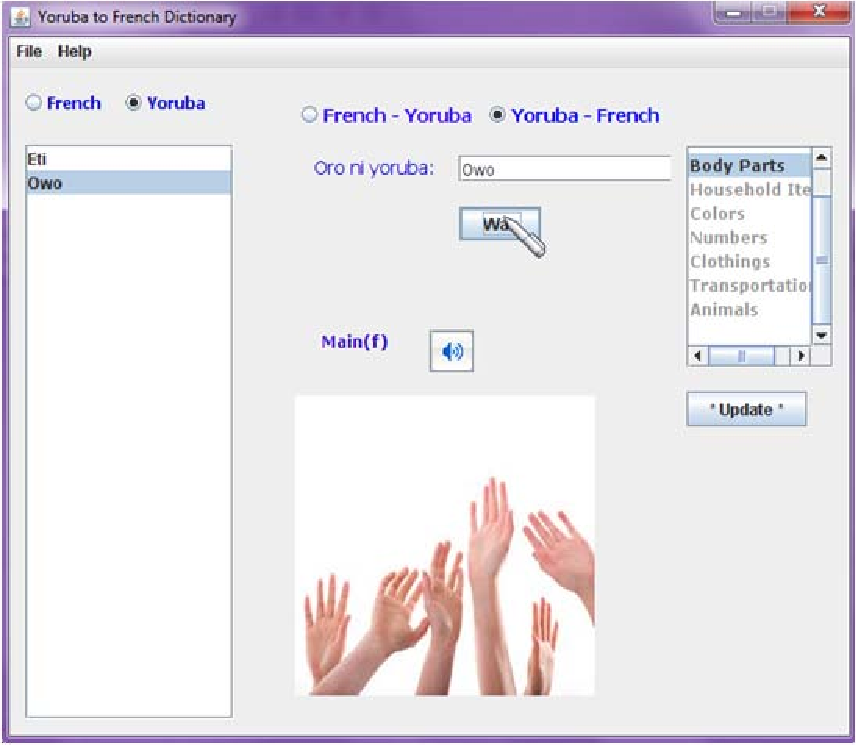
\includegraphics[scale=0.8]{dict2}
	\caption{Implementation Interface}
	\label{dict2l}
\end{figure}


Image of hardware implementation can be included as shown in Figure \ref{BreadbodaDiag}.
  

\begin{figure}[!h]
	\centering
	\fbox{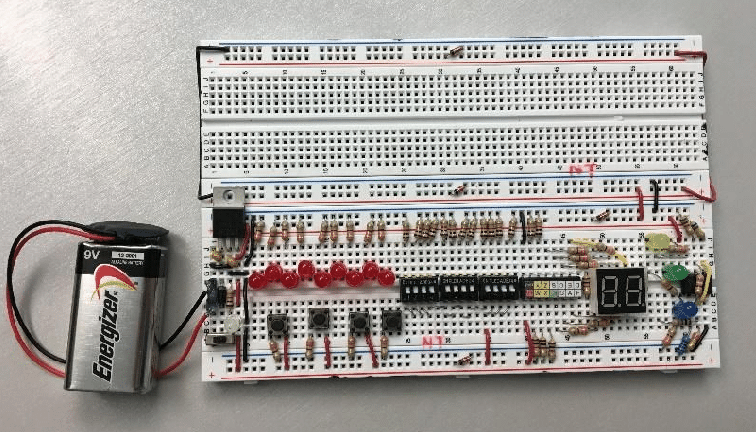
\includegraphics[scale=0.5]{Breadboard-Design-by-2}}
	\caption{Breadboard of hardware system implementation}
	\label{BreadbodaDiag}
\end{figure}


\section{System Evaluation} You are now to document in details  how you did your evaluation e.g.  alpha-beta method, mean-opinion score, hardware performance characteristics, etc. 





\section{Chapter Summary}

Summary of the contents of this chapter.
